\documentclass[12pt]{article}
\usepackage{amsmath,amssymb,graphicx,multicol,enumitem,amsthm}
\usepackage[margin=.5in]{geometry}
\pagestyle{empty}
\newtheorem{innercustomthm}{Theorem}
\newtheorem*{cor}{Corollary}
\newenvironment{thm}[1]
{\renewcommand\theinnercustomthm{#1}\innercustomthm}
{\endinnercustomthm}
\newcommand{\enumarabic}[1]{
	\begin{enumerate}[label=\textbf{\arabic*.}]
		#1
	\end{enumerate}
}
\newcommand{\enumalph}[1]{
\begin{enumerate}[label=(\alph*)]
	#1
\end{enumerate}
}
\theoremstyle{definition}
\newtheorem*{defn}{Definition}




%%%%%%%%%%
%Custom Commands
%%%%%%%%%%
\newcommand{\C}{\mathbb{C}}
\newcommand{\N}{\mathbb{N}}
\newcommand{\Q}{\mathbb{Q}}
\newcommand{\R}{\mathbb{R}}
\newcommand{\Z}{\mathbb{Z}}

\newcommand{\ds}{\displaystyle}

\newcommand{\fn}{\insertframenumber}

\newcommand{\im}{\operatorname{im}}

\newcommand{\blank}[1]{\underline{\hspace*{#1}}}

\newcommand{\abar}{\overline{a}}
\newcommand{\bbar}{\overline{b}}
\newcommand{\cbar}{\overline{c}}

\usepackage{tikz}
\usetikzlibrary{shapes.geometric}

\tikzset{
	buffer/.style={
		draw,
		regular polygon,
		regular polygon sides=3,
		fill=white,
		node distance=2cm,
		minimum height=4in,
		line width = 5pt
	}
}
\tikzset{
smaller/.style={
		draw,
		regular polygon,
		regular polygon sides=3,
		fill=white,
		node distance=2cm,
		minimum height=1in,
		line width = 2pt
	}
}
\tikzset{
square/.style={
	draw,
	regular polygon,
	regular polygon sides=4,
	fill=white,
	node distance=2cm,
	minimum height=4in,
	line width = 5pt
}
}
\tikzset{
smsquare/.style={
	draw,
	regular polygon,
	regular polygon sides=4,
	fill=white,
	node distance=2cm,
	minimum height=1in,
	line width = 2pt
}
}

\begin{document}
			\noindent Math 425: Abstract Algebra I
		
		\noindent	Symmetries of Regular $n$-gons
\vskip .25in


\noindent\textbf{Part 1: Symmetries of a Regular Triangle}

\noindent Instructions: Cut yourself a triangle that is this same shape and size. (One is provided on the last page of this document.)
Label its vertices (corners) with the numbers 1, 2, 3 on both the front and the back.\\
\begin{minipage}{3.5in}
	
	\noindent In class, we're going to explore the symmetries of this triangle (a regular 3-gon).  The group of which is called $D_3$.
	
	
	\noindent Let $r=$ clockwise rotation by 120$^\circ$ and $f=$ flip along the vertical axis.
	
	\noindent Note that we can think of these $r$ and $f$ as permutations of $\{1,2,3\}$.
	
	\noindent For example, consider $r$, then using two-line notation we have.
	\begin{center}
		\begin{minipage}{1.5in}
			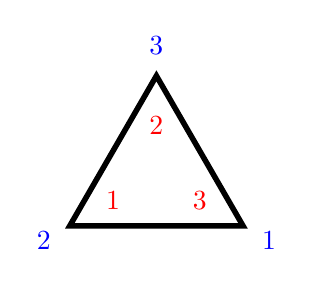
\begin{tikzpicture}
			\node[smaller]{};
			\node at (90:.65in) {\color{blue} 3};
			\node at (210:.65in) {\color{blue} 2};
			\node at (330:.65in) {\color{blue} 1};
			\node at (90:.25in) {\color{red} 2};
			\node at (210:.25in) {\color{red} 1};
			\node at (330:.25in) {\color{red} 3};
			\end{tikzpicture}
		\end{minipage}
		\begin{minipage}{1.5in}
			$\leftrightarrow$\quad
			$\ds r= \begin{pmatrix}
			\color{red} 1&\color{red} 2&\color{red} 3\\
			\color{blue}2&\color{blue} 3&\color{blue} 1
			\end{pmatrix}$
		\end{minipage}
	\end{center}
\end{minipage}
\begin{minipage}{4in}
	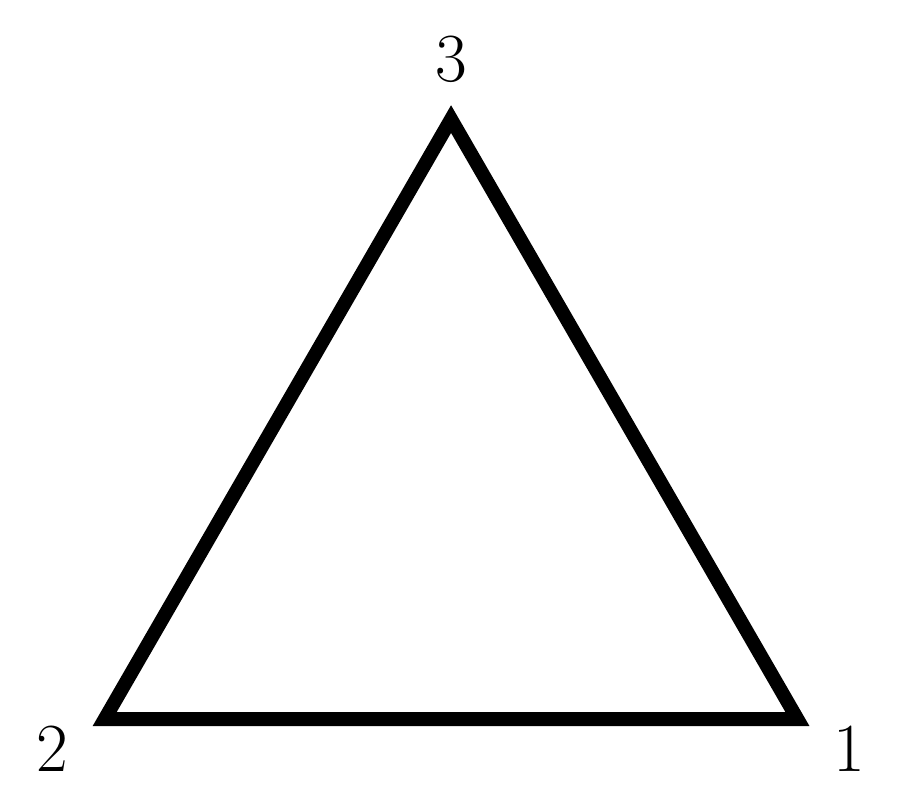
\begin{tikzpicture}
\node[buffer]{};
\node at (90:2.3in) {\Huge 3};
\node at (210:2.3in) {\Huge 2};
\node at (330:2.3in) {\Huge 1};
\end{tikzpicture}
\end{minipage}
Let's complete the following table
$$\large \begin{array}{|c|c|c|p{1.25in}|}
\hline
Elt&Two-line&cycle&$Symmetry$\\\hline
e&\begin{pmatrix}
1&2&3\\1&2&3
\end{pmatrix}&\varepsilon&do nothing\\\hline
r&\begin{pmatrix}
1&2&3\\2&3&1
\end{pmatrix}&(1\ 2\ 3)&$120^\circ$ clockwise\\\hline
r^2&\begin{pmatrix}
1&2&3\\&&
\end{pmatrix}&&\\\hline
\end{array}
\quad
\begin{array}{|c|c|c|p{1.25in}|}
	\hline
	Elt&Two-line&cycle&$Symmetry$\\\hline
	f&\begin{pmatrix}
		1&2&3\\&&
	\end{pmatrix}&&\\\hline
	fr&\begin{pmatrix}
		1&2&3\\&&
	\end{pmatrix}&{\color{white}(1\ 2\ 3)}&\\\hline
	fr^2&\begin{pmatrix}
		1&2&3\\&&
	\end{pmatrix}&&\\\hline
\end{array}
$$
\begin{enumerate}
	\item Did we miss any other symmetries? Why or why not? Is this set of symmetries equal to $S_3$?\vfill
	\item Use your cut-out triangle to find the symmetry $r^2frf^3r^4f$, in 2-line notation $\ds\begin{pmatrix}
	1&2&3\\&&
	\end{pmatrix}$.\vfill
	\item Use your cut-out triangle to prove that $f^2=e$, $r^3=e$, and $frf=r^2$.\vfill
	\item Use the identities in question 3 to reduce $r^2frf^3r^4f$ to $r^2f$.  Can you use an identity to make $r^2f$ look like one of the 6 symmetries in the table?\vfill
\end{enumerate}
\newpage
\noindent\textbf{Part 2: Symmetries of a Regular Rectangle (aka Square)}

\noindent Instructions: Cut yourself a square that is this same shape and size. (One is provided on the last page of this document.)
Label its vertices (corners) with the numbers 1, 2, 3, 4 on both the front and the back.\\
\begin{minipage}{3.5in}
\noindent In class, we're going to explore the symmetries of this square (a regular 4-gon).  The group of which is called $D_4$.


\noindent Let $r=$ clockwise rotation by 90$^\circ$ and $f=$ flip along the vertical axis.

\noindent Note that we can think of these $r$ and $f$ as permutations of $\{1,2,3,4\}$.

\noindent For example, consider $r$, then using two-line notation we have.
\begin{center}
	\begin{minipage}{1.5in}
		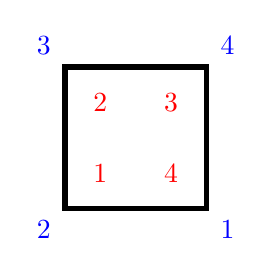
\begin{tikzpicture}
		\node[smsquare]{};
		\node at (45:.65in) {\color{blue} 4};
		\node at (135:.65in) {\color{blue} 3};
		\node at (225:.65in) {\color{blue} 2};
		\node at (315:.65in) {\color{blue} 1};
		\node at (45:.25in) {\color{red} 3};
		\node at (135:.25in) {\color{red} 2};
		\node at (225:.25in) {\color{red} 1};
		\node at (315:.25in) {\color{red} 4};
		\end{tikzpicture}
	\end{minipage}
	\begin{minipage}{1.75in}
		$\leftrightarrow$\quad
		$\ds r= \begin{pmatrix}
		\color{red} 1&\color{red} 2&\color{red} 3&\color{red}4\\
		\color{blue}2&\color{blue} 3&\color{blue} 4&\color{blue} 1
		\end{pmatrix}$
	\end{minipage}
\end{center}
\end{minipage}
\quad\quad
\begin{minipage}{4in}
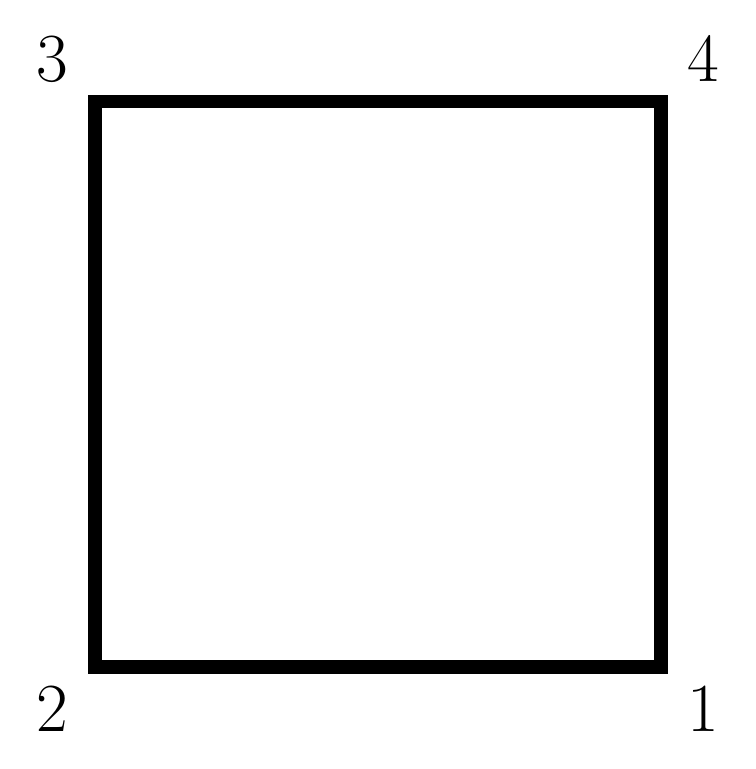
\begin{tikzpicture}
\node[square]{};
\node at (45:2.3in) {\Huge 4};
\node at (135:2.3in) {\Huge 3};
\node at (225:2.3in) {\Huge 2};
\node at (315:2.3in) {\Huge 1};
\end{tikzpicture}
\end{minipage}
Let's complete the following table
$$ \begin{array}{|c|c|c|p{1.25in}|}
\hline
Elt&Two-line&cycle&$Symmetry$\\\hline
e&\begin{pmatrix}
1&2&3&4\\1&2&3&4
\end{pmatrix}&\varepsilon&do nothing\\\hline
r&\begin{pmatrix}
1&2&3&4\\2&3&4&1
\end{pmatrix}&(1\ 2\ 3\ 4)&$90^\circ$ clockwise\\\hline
r^2&\begin{pmatrix}
1&2&3&4\\&&
\end{pmatrix}&&\\\hline
r^3&\begin{pmatrix}
1&2&3&4\\&&
\end{pmatrix}&&\\\hline
\end{array}
\quad
\begin{array}{|c|c|c|p{1.25in}|}
\hline
Elt&Two-line&cycle&$Symmetry$\\\hline
f&\begin{pmatrix}
1&2&3&4\\&&
\end{pmatrix}&&\\\hline
fr&\begin{pmatrix}
1&2&3&4\\&&
\end{pmatrix}&{\color{white}(1\ 2\ 3\ 4)}&\\\hline
fr^2&\begin{pmatrix}
1&2&3&4\\&&
\end{pmatrix}&&\\\hline
fr^3&\begin{pmatrix}
1&2&3&4\\&&
\end{pmatrix}&&\\\hline
\end{array}
$$
\begin{enumerate}
\item Did we miss any other symmetries? Why or why not? Is this set of symmetries equal to $S_4$?\vfill
\item Use your cut-out square to find the symmetry $rfrfr^{-3}$, in 2-line notation $\ds\begin{pmatrix}
1&2&3&4\\&&
\end{pmatrix}$.\vfill
\item Use your cut-out square to prove that $f^2=e$, $r^4=e$, and $frf=r^3$.\vfill
\item Use the identities in question 3 to reduce $rfrfr^{-1}$ to $r$.  \vfill
\item Is $fr^3f=r=r^{-3}$? Is $fr^2f=r^2=r^{-1}$? Make a conjecture about $fr^if$ for $i\in\Z$.\vfill
\end{enumerate}

\newpage
\noindent\textbf{PRINT AND CUT} Then duplicate the numbers on the reverse side of the shape too.
\vskip 1in
\begin{center}
	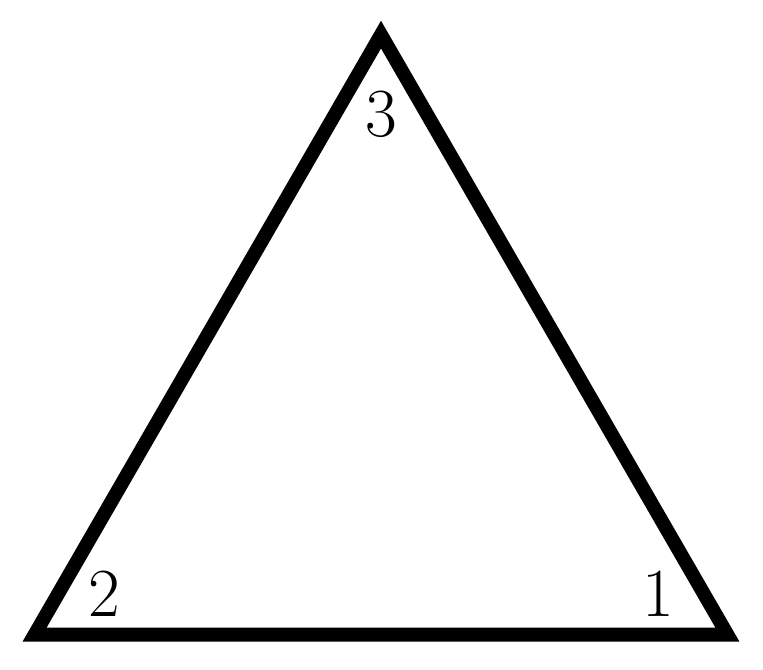
\begin{tikzpicture}
	\node[buffer]{};
	\node at (90:1.6in) {\Huge 3};
	\node at (210:1.6in) {\Huge 2};
	\node at (330:1.6in) {\Huge 1};
	\end{tikzpicture}
	\vskip 1in
	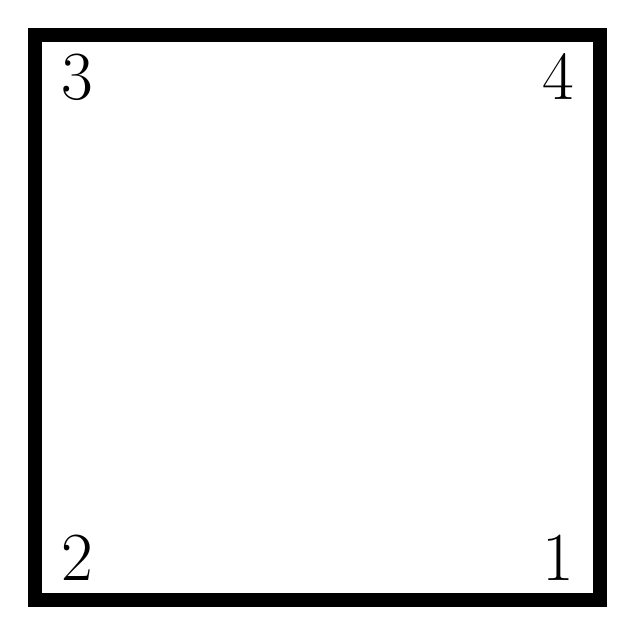
\begin{tikzpicture}
	\node[square]{};
	\node at (45:1.7in) {\Huge 4};
	\node at (135:1.7in) {\Huge 3};
	\node at (225:1.7in) {\Huge 2};
	\node at (315:1.7in) {\Huge 1};
	\end{tikzpicture}
\end{center}
\end{document}
